%! TEX program = lualatex

% Use :VimtexToggleMain to compile this file alone with Vimtex
\documentclass[tikz]{standalone}

\usepackage{sty/adantikz}

\begin{document}
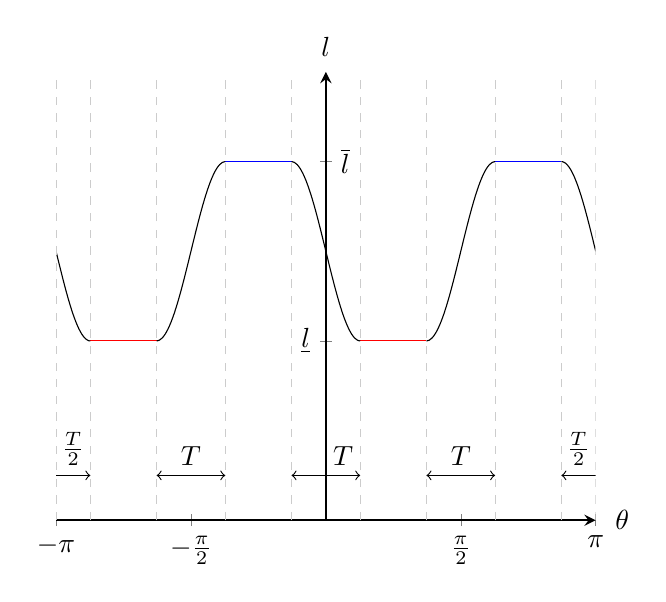
\begin{tikzpicture}
% Set the T variable
\pgfmathsetmacro{\T}{0.8}
% Set the underline{l} and overline{l} positions
\pgfmathsetmacro{\lu}{2}
\pgfmathsetmacro{\lb}{4}
\pgfmathsetmacro{\dl}{(\lb - \lu)/2}
\pgfmathsetmacro{\lavg}{(\lb + \lu)/2}
\pgfmathsetmacro{\w}{pi/\T}
% Define the figure
\begin{axis}[ 
 axis line style = thick,
 % Set the axes to be centered nicely
 axis x line = center, 
 axis y line = middle,
 xlabel = $\theta$, 
 x label style={at={(axis description cs:1.08,0)},anchor = east},
 xmin = -3.1415, xmax = 3.1415,
 ylabel = $l$,
 y label style={at={(axis description cs:0.5,1.1)},anchor = north}, 
 ymin = 0, ymax = 5,
 % Custom tick labels at specified positions
 xticklabels = {$-\pi$, $-\frac{\pi}{2}$, $0$, $\frac{\pi}{2}$, $\pi$},
 xtick={-3.1415, -1.571, 0, 1.571, 3.1415},
 yticklabels = {$\underline{l}$,$\overline{l}$},
 ytick = {\lu,\lb}, % Choose the plot values for underline{l} and overline{l}
 % Move the \overbar{l} label to the right
 yticklabel style={xshift={(\ticknum == 1)*(0.5cm)}}
]
    % Draw the l(theta) function's horizontal lines
    \addplot[red,domain=(-pi+(\T/2)):(-pi/2-(\T/2)),smooth]{\lu};
    \addplot[blue,domain=(-pi/2+(\T/2)):(-(\T/2)),smooth]{\lb};
    \addplot[red,domain=(\T/2):(pi/2-(\T/2)),smooth]{\lu};
    \addplot[blue,domain=(pi/2+(\T/2)):(pi-(\T/2)),smooth]{\lb};
    % Draw The l_(theta) sinusoids
    % Note that whatever expansions I've done is to prevent BadBox errors, and
    % should not be simplified (e.g. don't use deg() to convert to degrees, keep
    % minimal braces, etc)
    \addplot[black,domain=(-pi):(-pi+(\T/2)),smooth]{-\dl*sin(\w*x*180/pi+\w*180)+\lavg};
    \addplot[black,domain=(-pi/2-(\T/2)):(-pi/2+(\T/2)),smooth]{\dl*sin(\w*x*180/pi+\w*90) + \lavg};
    \addplot[black,domain=(-\T/2):(\T/2),smooth]{-\dl*sin(\w*x*180/pi)+\lavg};
    \addplot[black,domain=(pi/2-\T/2):(pi/2+\T/2),smooth]{\dl*sin(\w*x*180/pi-\w*90)+\lavg};
    \addplot[black,domain=(pi-\T/2):(pi),smooth]{-\dl*sin(\w*x*180/pi-\w*180)+\lavg};

    % Draw the vertical dashed lines at -pi
    \draw[dashed, color=gray!40] (-pi,0) -- (-pi,5);
    \draw[dashed, color=gray!40] (-pi+\T/2,0) -- (-pi+\T/2,5);
    \draw[->] (-pi,0.5) -- (-pi+\T/2,0.5) node[midway,above]{$\frac{T}{2}$};
    % Draw the vertical dashed lines at theta ~= - pi/2
    \draw[dashed, color=gray!40] (-pi/2-\T/2,0) -- (-pi/2-\T/2,5);
    \draw[dashed, color=gray!40] (-pi/2+\T/2,0) -- (-pi/2+\T/2,5);
    \draw[<->] (-pi/2-\T/2,0.5) -- (-pi/2+\T/2,0.5) node[midway,above]{$T$};
    % Draw the vertical dashed lines at 0
    \draw[dashed, color=gray!40] (-\T/2,0) -- (-\T/2,5);
    \draw[dashed, color=gray!40] (\T/2,0) -- (\T/2,5);
    \draw[<->] (-\T/2,0.5) -- (\T/2,0.5) node[above] at (0.2,0.5) {$T$};
    % Draw the vertical dashed lines at pi/2
    \draw[dashed, color=gray!40] (pi/2-\T/2,0) -- (pi/2-\T/2,5);
    \draw[dashed, color=gray!40] (pi/2+\T/2,0) -- (pi/2+\T/2,5);
    \draw[<->] (pi/2-\T/2,0.5) -- (pi/2+\T/2,0.5) node[midway,above]{$T$};
    % Draw the dashed lines at pi
    \draw[dashed, color=gray!40] (pi,0) -- (pi,5);
    \draw[dashed, color=gray!40] (pi-\T/2,0) -- (pi-\T/2,5);
    \draw[->] (pi,0.5) -- (pi-\T/2,0.5) node[midway,above]{$\frac{T}{2}$};
\end{axis}

\end{tikzpicture}
\end{document}
% vim: set tw=80 ts=4 sw=4 sts=0 et ffs=unix :
